\chapter{Preliminary evaluation of RTOS for RISC-V Based Hardware Accelerators}
\label{chapter:PreliminaryWork}
\section{Introduction}
% introdução ao trabalho que vou fazer
As mentioned in Chapter \ref{chapter:introduction} the purpose of this thesis is to evaluate the impact of a RTOS in the implementation of a RISC-V based hardware accelerator. To do this, it's necessary to develop the RTOS tasks that manage the use of the accelerator. After that, it's important to analyze the impacts of the RTOS on the overall system's performance and adjust the system according to those observations. It is also important to study how the system will scale with the complexity of the problem.



\section{Integrating a Hardware Accelerator in a RTOS}
% Como é que o rtos vai ajudar com o acelarador?
% falar de alguns métodos que posso usar para incorporar o acelarador no rtos (reunião 2023/05/05)
Typically, when using hardware accelerators to improve processing performance, the CPU has to wait for the accelerator to finish it's job before continuing with it's execution. This results in a waste of processing time in the CPU since it will stay waiting for the accelerator to finish its work. One way to improve this is to implement a system that uses the CPU's resources while the accelerator is performing its work. The use of a RTOS should make this management much easier.

A first naive solution to be explored is to make the task that started the accelerator sleep, freeing the CPU to work on other tasks, as can be seen in the block diagram in Figure \ref{fig:simpleImpl}. In this solution, the accelerator will have to wake the sleeping task by triggering an event or interrupt. This interrupt is then perceived by the ISR that, in turn, will change the state of the task that needs the data from the hardware accelerator.

\begin{figure}[H]
    \centering
    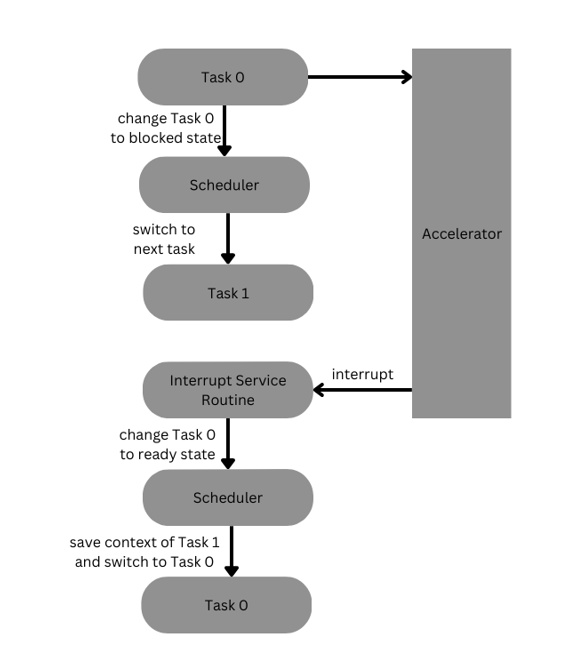
\includegraphics[scale=0.4]{Figures/simpleImpl.png}
    \caption{Block diagram of a first naive implementation}
    \label{fig:simpleImpl}
\end{figure}

Another solution is to have a specific task that manages the hardware accelerator. This task sits idle waiting to make use of the accelerator. Whenever other tasks need to use the accelerator they just need to communicate with the task that controls it and wait for the results.


\section{Preliminary Work}
% O que já fiz?
% Como é que o que já fiz ajuda o trabalho final?
The RVfpgaSoC \cite{RVfpgaSoC} course was followed to better understand the development cycle of the chosen RISC-V SoC, SweRVolfX. This course has a set of five labs to help build the SoC from scratch. The SoC designed was a subset of the one seen in Figure \ref{fig:SweRVolf}, except that the SPI1, SPI2, PTC and UART blocks were omitted for simplicity.

\begin{figure}[h]
    \centering
    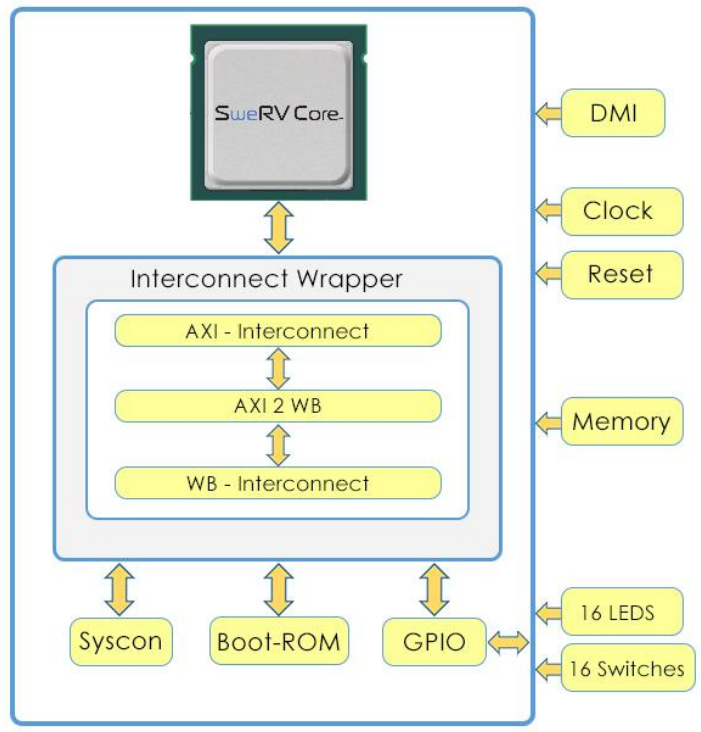
\includegraphics[scale=0.7]{Figures/SweRVolf.png}
    \caption{SweRVolf block diagram from the RVfpgaSoC course}
    \label{fig:SweRVolf}
\end{figure}

The most relevant labs were lab one, with an introduction to RVfpga and a guide on how to design the SoC using the Vivado Block Design Tool \cite{Vivado}, lab 2, with a guide on how to simulate the given examples using the tools verilator \cite{Verilator} and PlatformIO \cite{platformio} and lab 4, with a guide on how to install ZephyrOS in the SoC. After following these guides and with the knowledge accumulated the RTOS FreeRTOS was also installed in the SoC. With both RTOS, example programs were installed to familiarize myself with the mechanisms of the RTOS.

% SE TIVER TEMPO DE FAZER: INSTALAR PROGRAMAS SIMPLES QUE USAM VÁRIAS THREADS E COMUNICAM ENTRE SI


\section{Conclusion}
% Quais vão ser as métricas de desempanho?
This Chapter provides a small report on the preliminary work done on this thesis. First, it describes two initial solutions for how the RTOS can utilize the hardware accelerator. After that there is a description on the steps and guides taken to target the SoC to the FPGA and to install the RTOS in the system.

The integration of a RTOS into a RISC-V based hardware accelerator requires an evaluation and analysis of performance metrics. These metrics should help to study the efficiency and resource utilization of the system. Some of the key performance metrics are: ROM and RAM utilized, context switching delay, interrupt latency, message passing delay, and overall speedup of the application. Some benchmarks will be created to better test these metrics.



% RD: isto é o mais importante. é o que temos vindo a discutir
% introdução - explicar os ensaios/avaliaçoes
% 1 fase - explicar a escolha e utilização do rtos
% 2 fase - quais foram as configurações e porque
% 3 fase - como ficou e métricas de desempanho